\chapter{Final System}
\section*{Description} 
The purpose of the project is to develop a simulation environment for robot assisted minimally invasive surgery (RAMIS) team training. A top-down comparison can been in \autoref{Fig:SceneTop}. The simulation needs to allow trainees to practice different tasks and scenarios that might occur during real surgery.
The simulation should allow up to five trainees and an instructor to be simultaneously in the same virtual operating room. In the room, trainees should have access to all the tools and equipment that would be available to them during real training.
The simulation allows trainees to move on short distance by walking or teleport for long distance movement. Objects in the simulation, such as tools and the robot, can be grabbed to carry and interact with. A comparison between the modelled robot and the real one can be seen in \autoref{Fig:FinishHim}. Post processing was used to create a outline to indicate interactibility as seen in \autoref{Fig:Grabering}. There are two types of Tools; hand tools and laparoscopic tools. The hand tools are used mainly by the first nurse assistant. The laparoscopic tools includes the camera and tools that can be attached to the arms. Trainees can interact with the robot by moving its arms to achieve optimal placement, which is required for proper functioning of the robot. Additionally, voice over IP service is implemented to support communication between the trainees. 


\begin{figure}
\centering
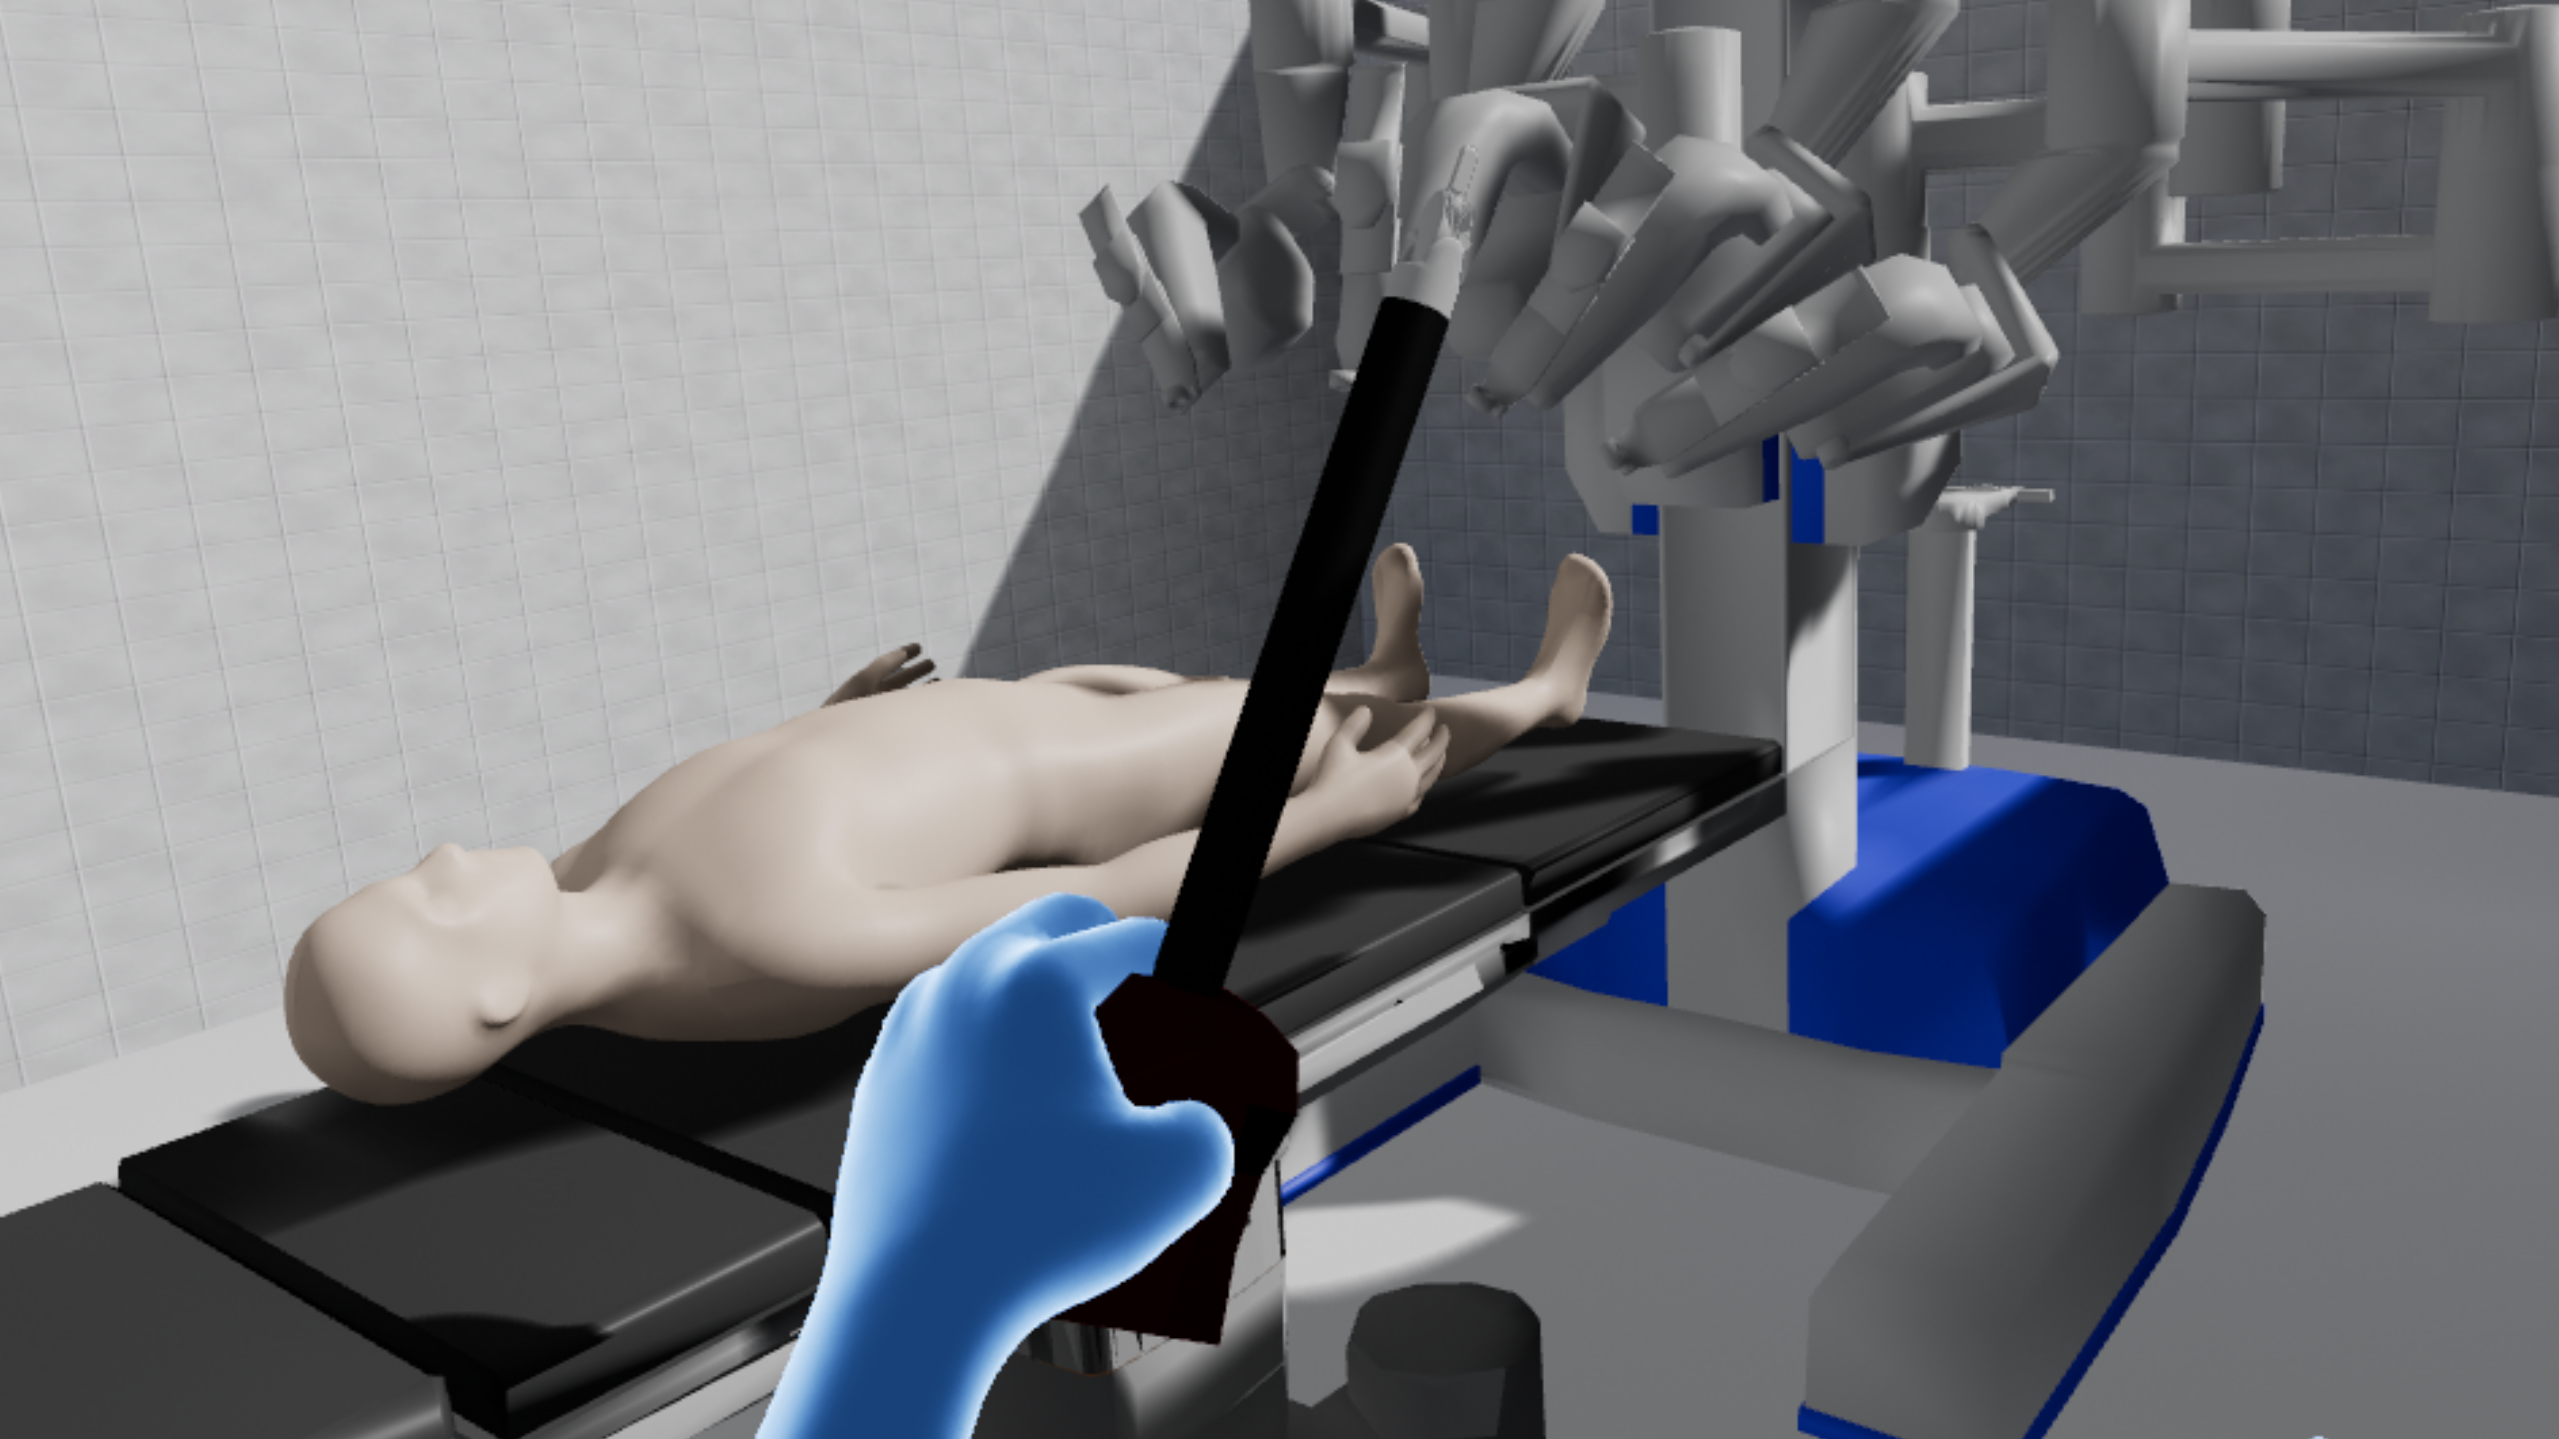
\includegraphics[width=0.45\textwidth]{FinishedSystem/RobInGame}
\includegraphics[width=0.45\textwidth]{FinishedSystem/RobIRL}
\caption{Left: Robot in the scene. Right: Robot in real life}
\label{Fig:FinishHim}
\end{figure}

\begin{figure}
\centering
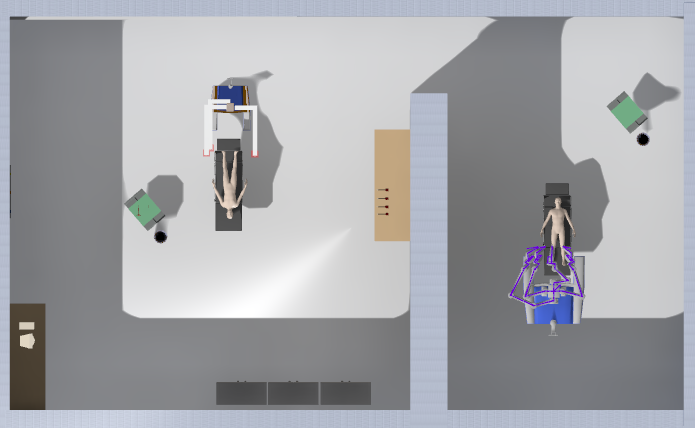
\includegraphics[width=0.45\textwidth]{FinishedSystem/SceneTop}
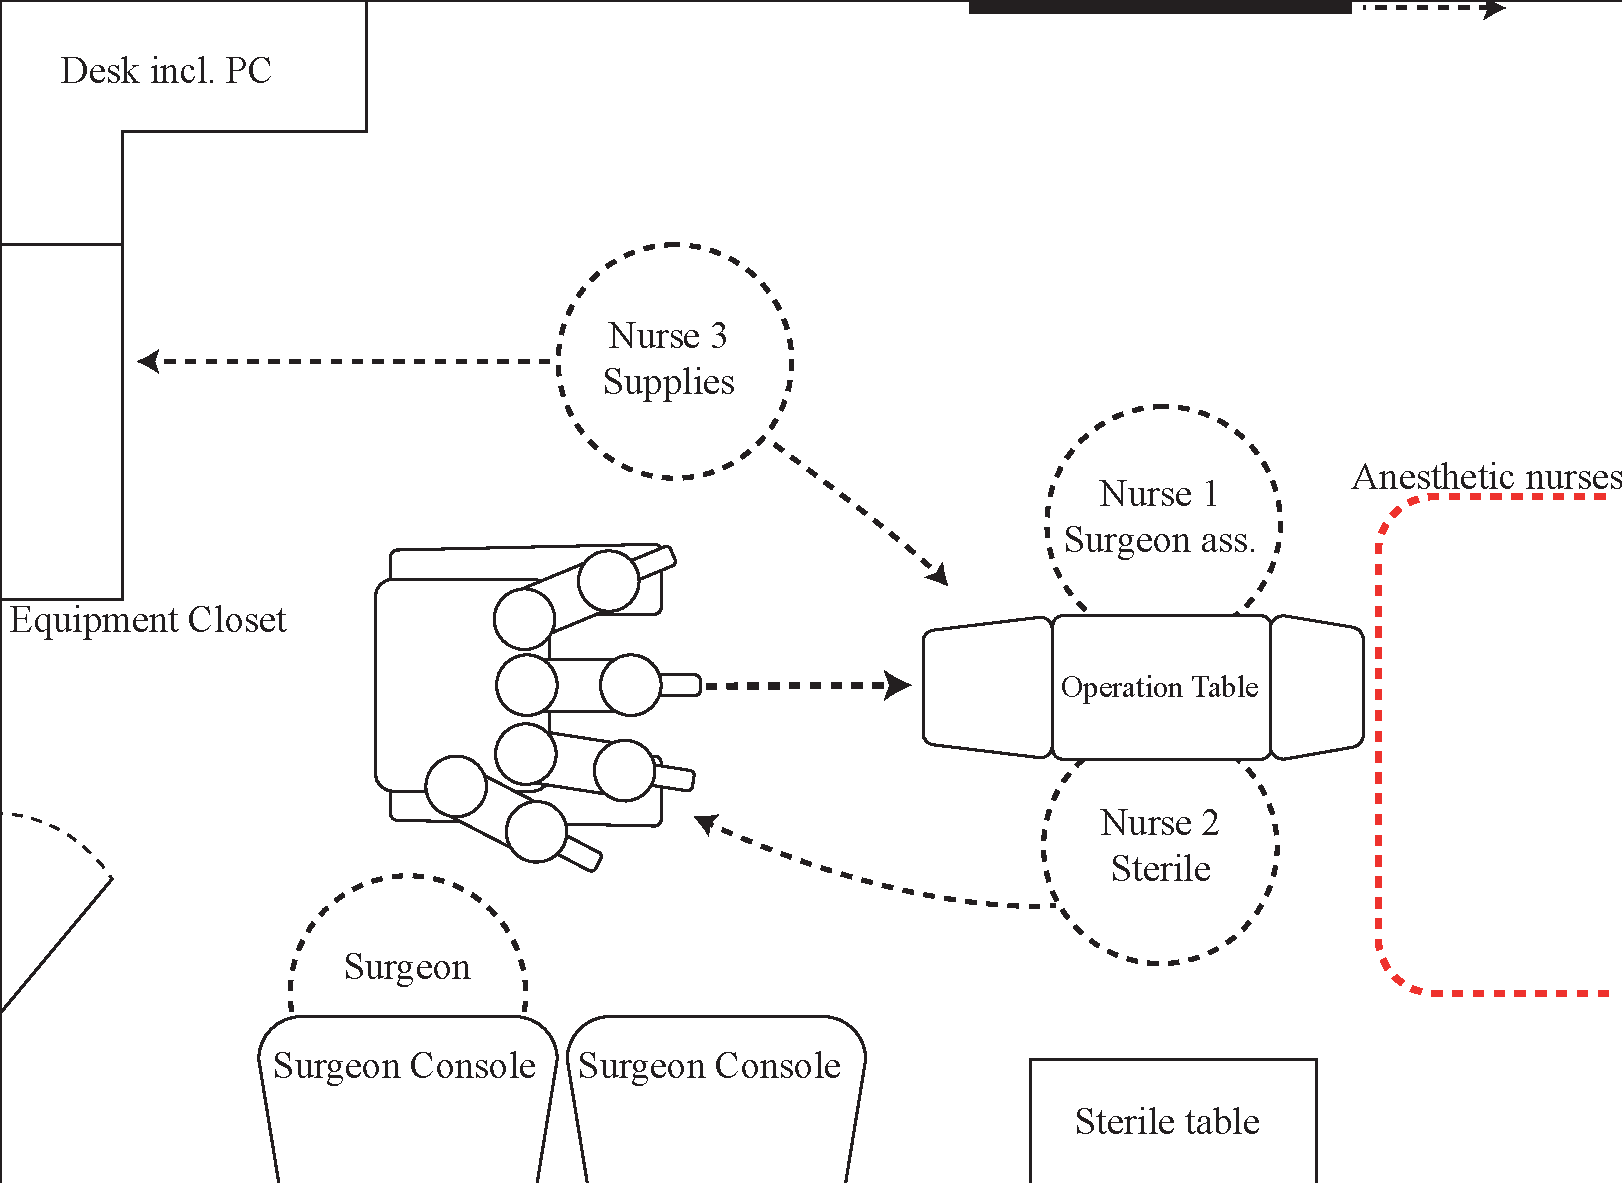
\includegraphics[width=0.45\textwidth]{FinishedSystem/overview_rotated}
\caption{Left: the scene in VR. Right: the physical operating room}
\label{Fig:SceneTop}
\end{figure}

\autoref{Fig:SceneTop} shows an overview of the scene as seen from above.

\begin{figure}
\centering
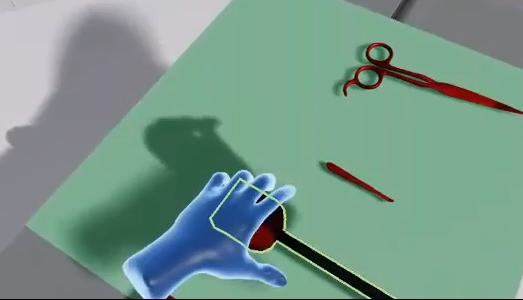
\includegraphics[width=0.75\textwidth]{FinishedSystem/grab}
\caption{The highlight feature when the user is within reach of an object}
\label{Fig:Grabering}
\end{figure}

